% SPDX-FileCopyrightText: Copyright (c) 2023-2025 Yegor Bugayenko
% SPDX-License-Identifier: MIT

\documentclass{article}
\usepackage{../lecture-notes/notes}
\newcommand*\thetitle{Maintainability Index}
\begin{document}

\lnTitlePage{5}{24}{xnSnPfVkmkM}

\plush{
  \pptPic{.6}{wtfs.png}}

\lnQuote
  [Fred Brooks]
  {fred-brooks}
  {The total \ul{cost of maintaining} a widely used program is typically 40 percent or more of the cost of developing it.}
  {brooks1978mythical}

\lnQuote
  [Richard G. Hamlet]
  {richard-hamlet}
  {It is a truism that \ul{good} software is easy to \ul{maintain}.}
  {hamlet1997}

\lnQuote
  [Ward Cunningham]
  {ward-cunningham}
  {Shipping first time code is like going into \ul{debt}. A little debt speeds development so long as it is paid back promptly with a rewrite. The danger occurs when the debt is not repaid. Every minute spent on not-quite-right code counts as interest on that debt.}
  {cunningham1992}

\lnQuote
  [Paul Oman]
  {anonymous}
  {Before developers can claim that they are building maintainable systems, there must be some way to \ul{measure} maintainability}
  {coleman1994}

\lnQuote
  {paper-1}
  {The factors of software that determine or influence maintainability can be organized into a \ul{hierarchical} structure of measurable attribute. Our hierarchy serves as a taxonomic definition for software maintainability that is compatible with the 35 published works upon which it is based.}
  {oman1992metrics}

\lnPitch{
  \pptBanner{Software Maintainability Taxonomy}
  \pptPic{.6}{tree.png}\par
  {\scriptsize Source: \bibentry{oman1992metrics}\par}}

\lnPitch{
  \pptBanner{Maintainability Formula}
  \begin{multicols}{2}
  \pptPic{.7}{formula-1.png}\par
  {\scriptsize Source: \bibentry{oman1992metrics}\par}
  \par\columnbreak\par
  ``This formula represents the product of the weighted dimensions, where each dimension is measured as the average deviation from a known value of 'goodness' for that maintainability attribute.''
  \end{multicols}}

\lnQuote
  {paper-2}
  {A software maintainability model is only useful if it can provide developers and maintainers in an industrial setting with more information about the system.}
  {coleman1994}

\lnPitch{
  \pptBanner{First Approximation}
  \begin{multicols}{2}
  \pptPic{.95}{formula-2.png}
  \par\columnbreak\par
  ``Approximately 50 regression models were constructed in an attempt to identify simple models that could be calculated from existing tools and still be generic enough to apply to a wide range of software systems. The regression model that seemed most applicable was a four-metric polynomial based on  \begin{inparaenum}[1)]\item Halstead’s effort, \item extended cyclomatic complexity, \item lines of code, and \item number of comments.\end{inparaenum}''
  \end{multicols}}

\lnPitch{
  \pptBanner{The Formula of Maintainability Index}
  \begin{multicols}{2}
  \pptPic{.95}{formula-3.png}
  \par\columnbreak\par
  \textit{aveVol} --- average Halstead Volume in a module\par
  \textit{ave V(g')} --- average total cyclomatic complexity in a module\par
  \textit{aveLOC} --- average lines of code in a module\par
  \textit{perCM} --- average percent of comments in a module\par
  \end{multicols}}

\lnPitch{
  \pptBanner{Maintainability Index by Visual Studio}
  \begin{multicols}{2}
  \pptPic{.95}{vs-formula.png}\par
  {\scriptsize Source: \href{https://radon.readthedocs.io/en/latest/intro.html}{Introduction to Code Metrics}, by Radon\par}
  \pptPic{.95}{vs-grades.png}\par
  {\scriptsize Source: \href{https://avandeursen.com/2014/08/29/think-twice-before-using-the-maintainability-index/}{Think Twice Before Using the ``Maintainability Index''}, by Arie van Deursen\par}
  \par\columnbreak\par
  ``We decided to be conservative with the thresholds. The desire was that if the index showed red then we would be saying with a high degree of confidence that there was an issue with the code.'' --- \href{https://learn.microsoft.com/en-us/visualstudio/code-quality/code-metrics-maintainability-index-range-and-meaning?view=vs-2022}{Code metrics --- Maintainability index range and meaning} by Microsoft, 2011.
  \end{multicols}}

\lnQuote
  [Rainer Niedermayr]
  {rainer-niedermayr}
  {We are convinced that Maintainability Index is \ul{nonsense}. We think that it is not sensible to reduce the maintainability of a whole software system to one single indicator.}
  {niedermayr2016}

\lnPitch{
  \pptThought{``The Maintainability Index does not provide information about the impact on development activities. A value of 57 does not express which maintainability aspects are affected by a bad value.'' --- Rainer Niedermayr}}

\lnQuote
  [Arie van Deursen]
  {arie-van-deursen}
  {If you are a researcher, \ul{think twice} before using the maintainability index in your experiments. Make sure you study and fully understand the original papers published about it.}
  {deursen2014}

\lnPitch{
  \pptThought{``Tool smiths and vendors used the exact same formula and coefficients as the 1994 experiments, without any recalibration.'' --- Arie van Deursen}}

\lnQuote
  [Tim Gilboy]
  {tim-gilboy}
  {If we're going to use the Maintainability Index we should use it to measure \ul{relative} maintainability within our project rather than use it as an \ul{absolute} metric.}
  {gilboy2022}

\lnPitch{
  \pptThought{\raggedright``Extending the length can significantly decrease Maintainability Index, even if all of the changes cause the code to be clearer and more understandable.'' --- Tim Gilboy}}

\lnQuote
  [Tja\u{s}a Heri\u{c}ko]
  {hericko}
  {When comparing maintainability measurements from several Index variants, the perception of maintainability could be impacted by the choice of the Index variant used.}
  {hericko2023}

\lnPitch{
  Maintainability Index is supported by a few tools:
  \begin{itemize}
  \item \href{https://visualstudio.microsoft.com/}{Visual Studio} for C++ and others
  \item \href{https://www.sonarsource.com/products/sonarqube/}{SonarQube} for Java
  \item \href{https://www.verifysoft.com/en_maintainability.html}{Testwell} for Java and C++ (not free)
  \item \href{https://radon.readthedocs.io/en/latest/index.html}{Radon} for Python
  \item \href{https://www.npmjs.com/package/jscomplexity}{jscomplexity} for JavaScript
  \item \href{https://github.com/yagipy/maintidx}{maintidx} for Go
  \end{itemize}}

\lnQuote
  {slr}
  {The SLR outcome provided us with \ul{174 software metrics}, among which we identified a set of 15 most commonly mentioned ones, and 19 metric computation tools available to practitioners.}
  {ardito2020tool}

\lnPitch{
  \begin{multicols}{2}
  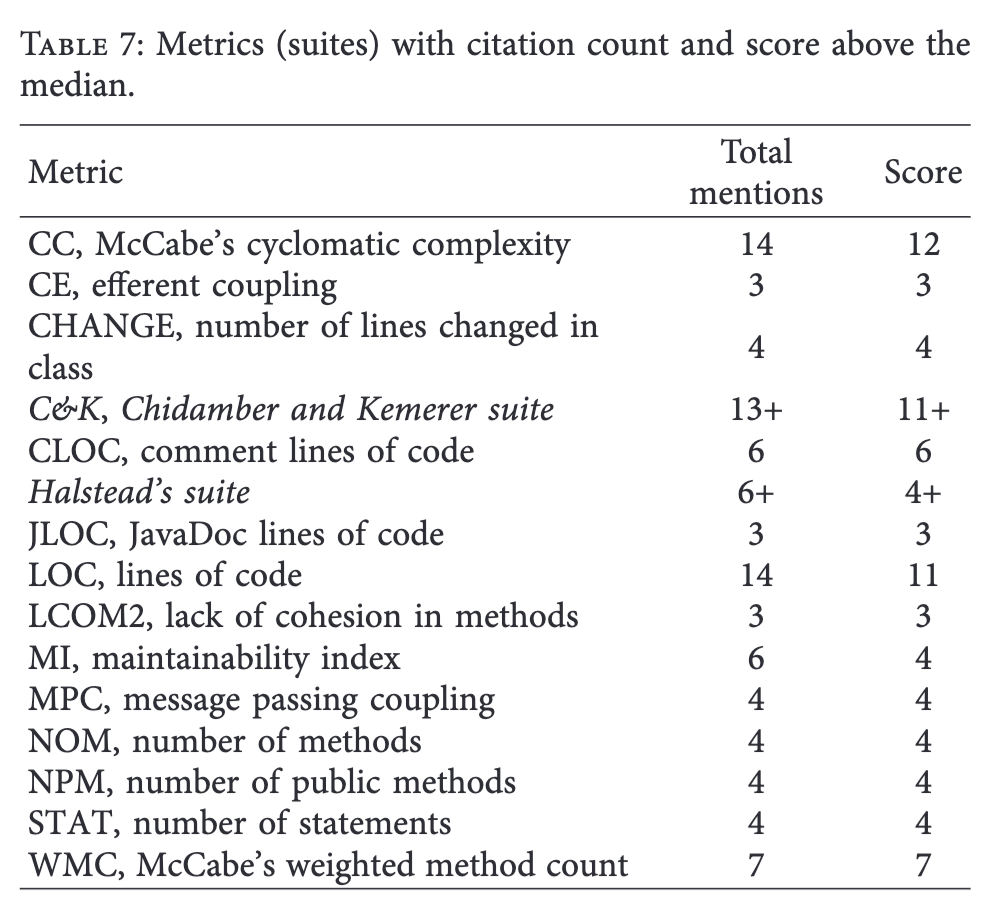
\includegraphics[width=.9\linewidth]{metrics.png}
  \par\columnbreak\par
  \lnSource{ardito2020tool}
  \end{multicols}}

\lnPitch{
  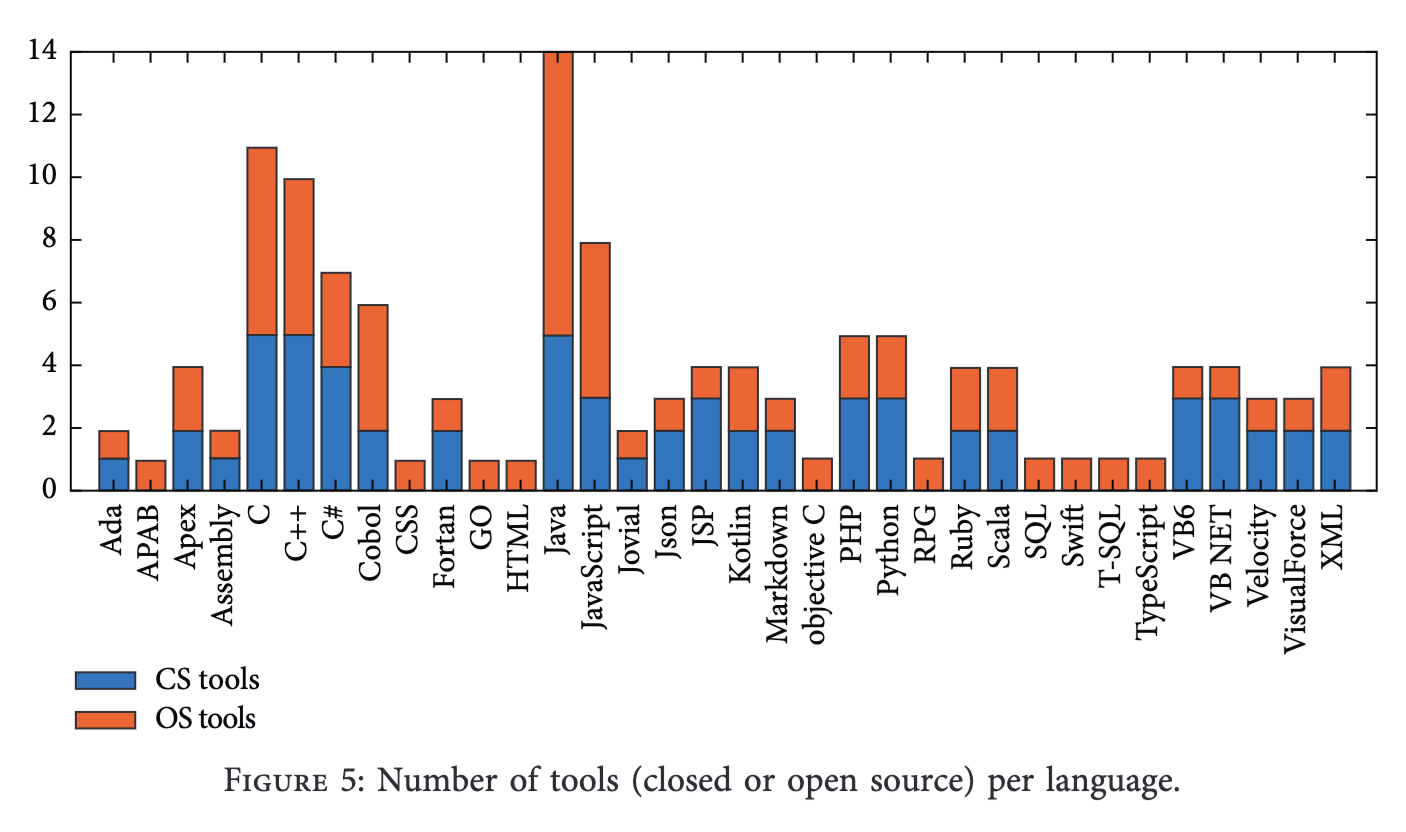
\includegraphics[width=.7\linewidth]{langs.png}\par
  \lnSource{ardito2020tool}}

% let's say something about "aggregation of software metrics"
% start from here: https://onlinelibrary.wiley.com/doi/abs/10.1002/smr.1558

\end{document}
